\chapter{Linear Regression}
A major component of machine learning, the one that most people associate with ML, is dedicated to making predictions under uncertain conditions. Given some input data, we would like to produce a target output. In this chapter, we're going to focus on the case where our prediction is a continuous, real number. This type of problem is known as \textbf{regression}.

\section{Introduction and Motivation}
It's important to emphasize that linear regression is just a subset of the larger class of techniques known as regression.

\begin{definition}{Regression}{regression}
A class of problems that seeks to make predictions about unknown target variables given observed input variables.
\end{definition}

\subsection{Examples of Regression}
We can imagine many situations where regression is useful:
\begin{enumerate}
    \item Predicting a person's height given the height of their parents.
    \item Predicting the probability that someone pays back a loan given their credit history.
    \item Predicting what time a package will arrive given current weather and traffic conditions.
\end{enumerate}

\subsection{Linear Regression}
In this chapter, we're specifically going to focus on \textbf{linear regression}, which means that our goal is to find some linear combination of the $x_{1}, ..., x_{D}$ input values that predict our target $y$.

\begin{definition}{Linear Regression}{linear-regression}
Suppose we have an input $\textbf{x}\in\mathbb{R}^D$ and a continuous target $y\in\mathbb{R}$.
Linear regression determines weights $w_{i}\in\mathbb{R}$ that balance the values of $x_{i}$ to produce $y$:
\begin{equation}
    y = w_{0} + w_{1}x_{1} + ... + w_{D}x_{D}
\end{equation}

\end{definition}

\readernote{Notice $w_{0}$ in the expression above, which doesn't have a corresponding $x_{0}$ value. This is known as the \textit{bias} term. If you consider the definition of a line $y = mx + b$, the bias term is comparable to the intercept $b$. It can account for a general trend in our data, such as if all of our target $y$ values are greater than 50.}

All of these follow a similar formula: a data input $\textbf{x}$ gets transformed into prediction $y$. For example, consider 10 year old Sam. She is curious about how tall she will be when she grows up. She has a data set of parents' heights and the final heights of their children. The inputs \textbf{x} are:
\begin{align*}
x_{1} = \text{height of mother (cm)} \\
x_{2} = \text{height of father (cm)}
\end{align*}
Using linear regression, she determines the weights \textbf{w} to be:
\begin{align*}
\textbf{w} = [34, 0.39, 0.33] \\
\end{align*}
Sam's mother is 165 cm tall and her father is 185 cm tall. Using the results of the linear regression solution, Sam solves for her expected height:
\begin{align*}
\text{Sam's height} = 34 + 0.39(165) + 0.33(185) = \textbf{159.4 cm}
\end{align*}

\begin{mlcube}{Linear Regression}
Let's inspect the categories linear regression falls into for our ML framework cube. First, as we've already stated, linear regression deals with a \textbf{continuous} input and output domain. Second, our goal is to make predictions on future data points, and to construct something capable of making those predictions we first need a labeled data set of inputs and outputs. This makes linear regression is a \textbf{supervised} technique. Third and finally, linear regression is a special case when it comes to being \textbf{probabilistic or non-probabilistic}. Depending on our interpretation, it can be either one! We will explain how this works later in the chapter.
\begin{center}
    \begin{tabular}{c|c|c}
    \textit{\textbf{Domain}} & \textit{\textbf{Training}} & \textit{\textbf{Probabilistic}} \\
    \hline
    Continuous & Supervised & Yes / No \\
    \end{tabular}
\end{center}
\end{mlcube}

\section{Technical}
The most basic form of linear regression is a simple weighted combination of the input variables $\textbf{x}$, which you will often see written as:

\begin{equation}
    y(\textbf{x}, \textbf{w}) = w_{0} + w_{1}x_{1} + ... + w_{D}x_{D}
\end{equation}

\subsection{Merging of Bias}
We're going to introduce a common notational trick here for making the bias term, $w_{0}$, easier to handle. At the moment $w_{0}$ is unwieldly because it is not being multiplied by an $x_{i}$ value. Without the bias term, we could easily express $y(\textbf{x}, \textbf{w})$ as:
\begin{equation}
    y(\textbf{x}, \textbf{w}) = \textbf{w}^{T}\textbf{x} = w_{0}x_{0} + w_{1}x_{1} + ... + w_{D}x_{D}
\end{equation}
 This is more compact, easier to reason about, and makes properties of linear algebra nicer for the calculations we will be performing. An easy way to keep our bias term and still get this nice form of $\textbf{w}^{T}\textbf{x}$ is to simply introduce another variable, $x_{0}$, that is always $1$ for every data point. For example, considering the case of Sam's height from above, we have the height of her parents, \textbf{x}:
\begin{align*}
    \textbf{x} = (165, 185)
\end{align*}
We now add a $1$ in the first position of the data point to make it:
\begin{align*}
    \textbf{x'} = (1, 165, 185)
\end{align*}
We do this for every point in our data set. This bias trick lets us write:
\begin{equation}
    y(\textbf{x}, \textbf{w}) = \textbf{w}^{T}\textbf{x} = w_{0}x_{0} + w_{1}x_{1} + ... + w_{D}x_{D}
\end{equation}
as desired.

\subsection{Visualization of Linear Regression}
Let's try to build some intuition about how linear regression works. Our algorithm is provided with a collection of data points: inputs \textbf{x} and corresponding targets \textbf{y}. Our goal is to find the best set of weights \textbf{w} such that given a new data point \textbf{x}, we can accurately predict the true target value $y$. This is visualizable in the simple case where $\textbf{x}$ is a 1-dimensional input variable, as in Figure \ref{fig:simple-lin-reg}.

\begin{figure}
    \centering
    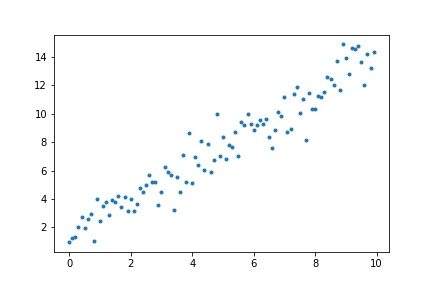
\includegraphics[width=0.5\paperwidth]{../LinearRegression/fig/simple_lin_reg_GEN.jpg}
    \caption{Data set with clear trend.}
    \label{fig:simple-lin-reg}
\end{figure}

Our eyes are naturally able to detect a very clear trend in this data. If we were to be given a new $\textbf{x}$ data point, how would be predict its target value $y$? We would first fit a line to our data, as in Figure \ref{fig:simple-lin-reg-w-line}, and then find where on that line the new $\textbf{x}$ value sits.

\begin{figure}
    \centering
    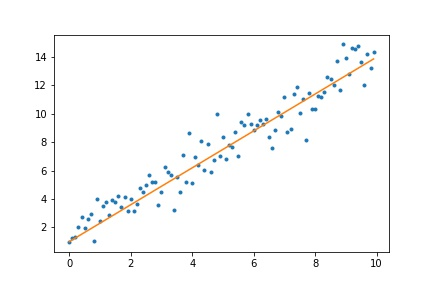
\includegraphics[width=0.5\paperwidth]{../LinearRegression/fig/simple_lin_reg_w_line_GEN.jpg}
    \caption{Data set with clear trend, best fitting line included.}
    \label{fig:simple-lin-reg-w-line}
\end{figure}

That is the entirety of linear regression! It fits the `best' line to our data, and then uses that line to make predictions. In 1-D input space, this manifests itself as the simple problem seen above, where we need only find a single bias term $w_{0}$ (which acts as the intercept of the line) and single weight $w_{1}$ (which acts as the slope of the line). However, the same principle applies to higher dimensional data as well. We're always fitting the line (meaning calculate the weights $\textbf{w}$) that give us maximal predictive power.

\readernote{Although our input data points $\textbf{x}$ can take on multiple dimensions, our output data $y$ is always a 1-dimensional real number when dealing with regression problems.}

Now that we have some intuition for what linear regression is, a natural question arises: how do we find these `best' values for $\textbf{w}$? That is the remaining focus of this chapter.

\subsection{Finding the Best Fitting Line: Loss}
We can inspect a set of data as presented in Figure \ref{fig:simple-lin-reg}, and are quite good at fitting a line by hand. When we fit that line, whether we think about it or not, what we're trying to do is make the line as close to all of the data points as possible. We can formalize this notion by introducing the concept of \textbf{loss}, and use it to our advantage in developing a method to automatically fit a line to our data.


\begin{definition}{Loss}{loss}
Loss is the error incurred for a given prediction. It can be thought of as a measurement of difference between the target ($t$) and predicted ($y(\textbf{x}, \textbf{w}$)) values:
\begin{align*}
    \mathcal{L}(\textbf{w}) = \text{target} - \text{prediction} = t - y(\textbf{x}, \textbf{w}) = \boxed{t - \textbf{w}^{T}\textbf{x}}
\end{align*}

Notice that loss is denoted $\mathcal{L}(\textbf{w})$, and it is a function of our parameters $\textbf{w}$, which are used to generate our prediction. Loss can be computed in different manners, and the choice of what loss function to use has important implications that we will discuss.
\end{definition}

Loss is a concept that we will come back to very frequently in the context of supervised machine learning methods.

\subsection{Least Squares Loss}
As we mentioned above, there are different methods for computing loss. One of the most commonly used measurements is known as \textbf{Least Squares Loss}. Least squares, as it is often abbreviated, says that the loss for a given data point is the square of the difference between the target and predicted values:
\begin{equation} \label{least-squares-loss-fn}
    \mathcal{L}(\textbf{w}) = (t - \textbf{w}^{T}\textbf{x})^2
\end{equation}
There is a satisfying statistical interpretation for using this loss function which we will explain later in this chapter, but for now it will suffice to discuss some of the properties of this loss function that make it desirable.

First, notice that it will always take on positive values. This is convenient because we can focus exclusively on minimizing our loss, and it also allows us to combine the loss incurred from different data points without worrying about them cancelling out.

A more subtle but enormously important property of this loss function is that we know a lot about how to efficiently optimize quadratic functions. This is not a textbook about optimization, but some quick and dirty intuition that we will take advantage of throughout this book is that we can easily and reliably take the derivative of a quadratic function because they are continuously differentiable. We also know that optima of a quadrative function will be located at points where the derivative of the function is equal to 0, as seen in Figure \ref{fig:quad-deriv-at-2}.

\begin{figure}
    \centering
    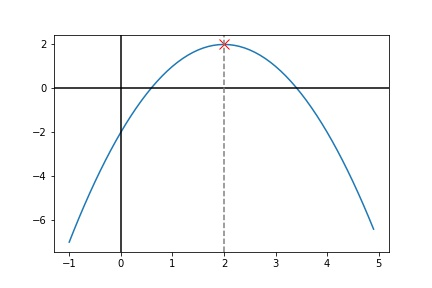
\includegraphics[width=0.5\paperwidth]{../LinearRegression/fig/deriv_at_2_GEN.jpg}
    \caption{Quadratic function with clear optimum at $x=2$, where the derivative of the function is 0.}
    \label{fig:quad-deriv-at-2}
\end{figure}

If we compare this to an alternative loss function, such as an absolute value loss:
\begin{align}
    \mathcal{L}(\textbf{w}) = \lvert t - \textbf{w}^{T}\textbf{x} \rvert
\end{align}

We know that this function is not continuously differentiable around its optima, and as a result, it is much less convenient to work with as compared to least squares loss.

** add something about aversion to outliers using least squares loss? **
** add a visualization of what the loss actually looks like for a toy data set (small little red lines from predicted to true) **

\subsection{Optimal Weights via Matrix Differentiation}
Now that we have our least squares loss function, we can finally begin to fit a line to our data. First, we can define the loss incurred by parameters $\textbf{w}$ over our entire data set $\textbf{X}$ as follows:
\begin{align}
    \mathcal{L}(\textbf{w}) = \frac{1}{2} \sum_{i=1}^{n} (t - \textbf{w}^{T}\textbf{x})^2
\end{align}

\readernote{Note that we added a constant $\frac{1}{2}$ to the beginning of our loss expression. This scales the loss, which will not change our final result for the optimal parameters. It has the benefit our calculations cleaner once we've taken the gradient of the loss.}

We now want to solve for the values of $\textbf{w}$ that minimize this expression, since a small loss implies that we are doing a good job of predicting values that are close to their true target values.

\begin{derivation}{Least Squares Derivation}{least-squares-derivation}
    We find the optimal weights $\textbf{w}^{*}$ as follows: \\

    Start by taking the gradient of the loss with respect to our parameter $\textbf{w}$:
    \begin{align*}
        \nabla \mathcal{L}(\textbf{w}) = \sum_{i=1}^{n} (t - \textbf{w}^{T}\textbf{x})\textbf{x}^{T}
    \end{align*}

    Setting this gradient to 0, we have:
    \begin{equation} \label{least-squares-solving-for-w}
        0 = \sum_{i=1}^{n} t \textbf{x}^{T} - \textbf{w}^{T} \sum_{i=1}^{n} \textbf{x}\textbf{x}^{T}
    \end{equation}

    At this point, it is convenient to rewrite these summations as matrix operations in terms of $\textbf{w}$ instead of $\textbf{w}^{T}$. Note that $(\textbf{w}^{T} \sum_{i=1}^{n} \textbf{x}\textbf{x}^{T})^{T} = \textbf{X}^{T}\textbf{X}\textbf{w}$ and $(\sum_{i=1}^{n} t \textbf{x}^{T})^{T} = \textbf{X}^{T}\textbf{Y}$. Rewriting:
    \begin{align*}
        0 = \textbf{X}^{T}\textbf{Y} - \textbf{X}^{T}\textbf{X}\textbf{w}
    \end{align*}

    Solving for $\textbf{w}^{*}$:
    \begin{equation} \label{least-squares-solved-for-w}
        \textbf{w}^{*} = (\textbf{X}^{T}\textbf{X})^{-1}\textbf{X}^{T}\textbf{Y}
    \end{equation}
\end{derivation}

Note that the quantity $(\textbf{X}^{T}\textbf{X})^{-1}\textbf{X}^{T}$ in Derivation \ref{der:least-squares-derivation} has a special name: the \textbf{\textit{Moore-Penrose pseudo inverse}}. You can think of it as a generalization of a matrix inversion operation to a non-square matrix.

\subsection{Linear Regression as Projection}
Another common interpretation of linear regression is that of a projection of our targets, $\textbf{Y}$, onto the column space of our inputs $\textbf{X}$. This can be useful for building intuition.

We showed above that the quantity $(\textbf{X}^{T}\textbf{X})^{-1}\textbf{X}^{T}$ can be thought of as the pseudoinverse for our inputs $\textbf{X}$. Let's now consider the case where $\textbf{X}$ is square and the pseudoinverse is equal to the true inverse: $\textbf{X}^{-1} = (\textbf{X}^{T}\textbf{X})^{-1}\textbf{X}^{T}$. We have for our optimal $\textbf{w}^{*}$:
\begin{align*}
    \textbf{w}^{*} = (\textbf{X}^{T}\textbf{X})^{-1}\textbf{X}^{T}\textbf{Y}
\end{align*}
which becomes
\begin{align*}
    \textbf{w}^{*} = \textbf{X}^{-1}\textbf{Y}
\end{align*}
We can recover our target values $\textbf{Y}$ by multiplying either side by $\textbf{X}$:
\begin{align*}
    \textbf{X}\textbf{w}^{*} = \textbf{X}\textbf{X}^{-1}\textbf{Y} \\
    \textbf{X}\textbf{w}^{*} = \textbf{Y}
\end{align*}

We were able to recover our targets $\textbf{Y}$ exactly because $\textbf{X}$ is an invertible tranformation. However, in the general case where $\textbf{X}$ is not invertible and we have to use the approximate pseudoinverse $(\textbf{X}^{T}\textbf{X})^{-1}\textbf{X}^{T}$, we instead recover $\hat{\textbf{Y}}$:
\begin{align*}
    \textbf{X}\textbf{w}^{*} = \textbf{X}(\textbf{X}^{T}\textbf{X})^{-1}\textbf{X}^{T}\textbf{Y} \\
    \textbf{X}\textbf{w}^{*} = \hat{\textbf{Y}}
\end{align*}
where $\hat{\textbf{Y}}$ can be thought of as the closest projection of $\textbf{Y}$ into the column space of $\textbf{X}$. Furthermore, this motivates the intuition that $\textbf{w}^{*}$ is the set of coefficients that best transforms our input space $\textbf{X}$ into our target values $\textbf{Y}$.

\subsection{Basis Functions}
There are some situations where our input data $\textbf{X}$ is not the best form of our data for performing linear regression. Because linear regression only scales and combines input variables, it is unable to apply more complex transformations to our data such as a sin or squaring function. In those situations where we need to transform our input variable somehow prior to performing linear regression (which is known as moving our data into a new \textit{basis}, we apply what is known as a \textbf{basis function}.

\begin{definition}{Basis Function}{basis-fn}
    Typically denoted by the symbol $\phi(\cdot)$, a basis function is a transformation applied to an input data point $\textbf{x}$ to move our data into a different \textit{input basis}, which is another phrase for \textit{input domain}. \\

    For example, consider our original data point:
    \begin{align*}
        \textbf{x} = (x_{1}, x_{2})'
    \end{align*}
    We may choose our basis function $\phi(\textbf{x})$ such that our transformed data point in its new basis is:
    \begin{align*}
        \textbf{x} = (x_{1}, x_{1}^2, x_{2}, \sin{x_{2}})'
    \end{align*}

    Using a basis function is so common that we will sometimes describe our input data points as $\boldsymbol{\phi} = (\phi_{1}, \phi_{2}, ..., \phi_{D})'$.
\end{definition}

Basis functions are very general - they could specify that we just keep our input data the same. As a result, it's common to rewrite the least squares loss function from Equation \ref{least-squares-loss-fn} for linear regression in terms of the basis function applied to our input data:

\begin{equation} \label{least-squares-loss-fn-w-basis}
    \mathcal{L}(\textbf{w}) = \frac{1}{2} \sum_{i=1}^{n} (t - \textbf{w}^{T}\boldsymbol{\phi})^2
\end{equation}

To motivate why we might need basis functions for performing linear regression, let's consider this graph of 1-dimensional inputs \textbf{X} along with their target outputs \textbf{Y}, presented in Figure \ref{fig:lin-reg-no-basis-fn}.

\begin{figure}
    \centering
    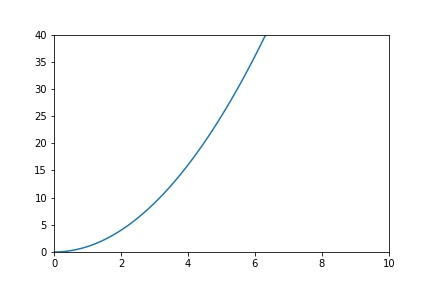
\includegraphics[width=0.5\paperwidth]{../LinearRegression/fig/lin_reg_no_basis_fn_GEN.jpg}
    \caption{Data with no basis function applied.}
    \label{fig:lin-reg-no-basis-fn}
\end{figure}

As we can see, we're not going to be able to fit a good line to this data. The best we can hope to do is something like that of Figure \ref{fig:lin-reg-no-basis-fn-fitted}.

\begin{figure}
    \centering
    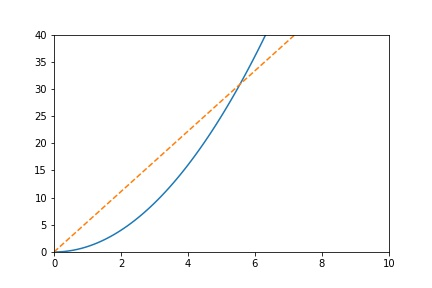
\includegraphics[width=0.5\paperwidth]{../LinearRegression/fig/lin_reg_no_basis_fn_fitted_GEN.jpg}
    \caption{Data with no basis function applied, attempt to fit a line.}
    \label{fig:lin-reg-no-basis-fn-fitted}
\end{figure}

However, if we just apply a simple basis function to our data, in this case the simple square root function, $\phi(\textbf{x}) = (\sqrt{x_{1}})'$, we now have the red line in Figure \ref{fig:lin-reg-w-basis-fn-fitted}.

\begin{figure}
    \centering
    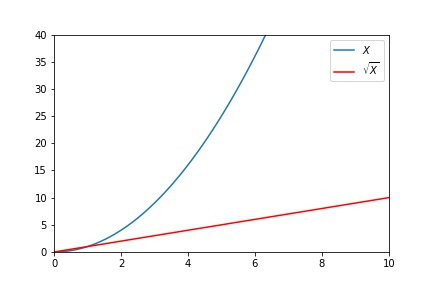
\includegraphics[width=0.5\paperwidth]{../LinearRegression/fig/lin_reg_w_basis_fn_GEN.jpg}
    \caption{Data with square root basis function applied.}
    \label{fig:lin-reg-w-basis-fn-fitted}
\end{figure}

We now see that we can fit a very good line to our data, thanks to basis functions. Still, the logical question remains: how can I choose the appropriate basis function? This toy example had a very obviously good basis function, but in general with high dimensional, messy input data, how do we choose the basis function we need?

The answer is that this is not an easy problem to solve. Often, you may have some domain specific knowledge that tells you to try a certain basis, such as if you're working with chemical data and know that an important equation involves a certain function of one of your inputs. However, more often than not we won't have this expert knowledge either. Later on, we will discuss methods for discovering the best basis functions for our data automatically.

\subsection{Regularization}
How we can mitigate the problem of overfitting, especially if we want to try a lot of basis functions
why we need it, different types, what its effects are
Now that we've introduced the idea of basis functions, you might wonder why we don't just try adding many basis transformations to our input data to find a good transformation. For example, we might use this large basis function:
\begin{align*}
    \phi(\textbf{x}) = (x_{1}, x_{1}^{2}, ..., x_{1}^{100}, x_{2}, x_{2}^{2}, ..., x_{2}^{100}, x_{D}, x_{D}^{2}, ..., x_{D}^{100})'
\end{align*}

all we've done is tried transforming every input data point up to 100 degrees. Can you imagine what might happen now that we've done this?

Let's say our input data point \textbf{x} is simply 1-dimensional, and we apply the basis function described above, so that after the transformation each data point is represented by 100 values. Say we have 100 data points on which to perform linear regression, and because our transformed input space has 100 values, we have 100 parameters to fit. In this case, with one parameter per data point, it's possible for us to fit our regression line perfectly to our data so that we have 0 loss! But is this a desirable outcome? The answer is no, and we'll provide a visual example to illustrate that.

Imagine Figure \ref{fig:data-set-scattered} is our data set.

\begin{figure}
    \centering
    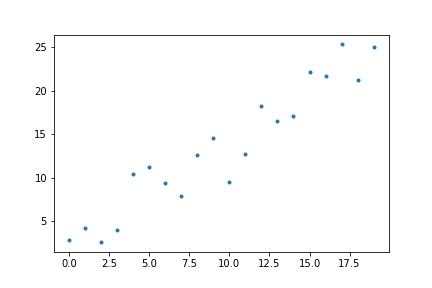
\includegraphics[width=0.5\paperwidth]{../LinearRegression/fig/data_set_scattered_GEN.jpg}
    \caption{Data set with a clear trend and Gaussian noise.}
    \label{fig:data-set-scattered}
\end{figure}

There is a very clear trend in this data, and you would likely draw a line that looks something like that of Figure \ref{fig:data-set-natural-fit} to fit it.

\begin{figure}
    \centering
    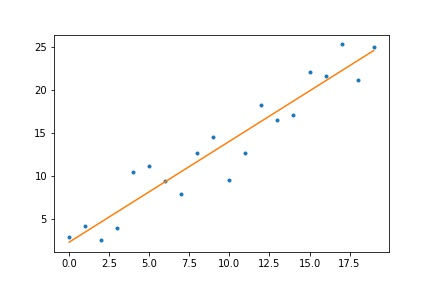
\includegraphics[width=0.5\paperwidth]{../LinearRegression/fig/data_set_natural_fit_GEN.jpg}
    \caption{Natural fit for this data set.}
    \label{fig:data-set-natural-fit}
\end{figure}

However, imagine now we performed a large basis transformation like the one described above. If we do that, it's possible for us to fit our line perfectly, threading every data point, like that in Figure \ref{fig:data-set-unnatural-fit}.

\begin{figure}
    \centering
    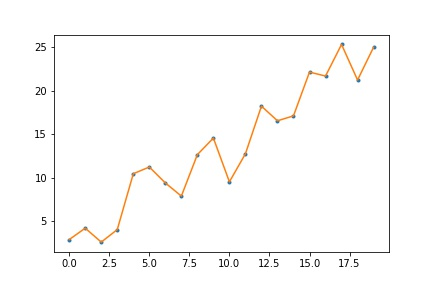
\includegraphics[width=0.5\paperwidth]{../LinearRegression/fig/data_set_unnatural_fit_GEN.jpg}
    \caption{Unnatural fit for this data set.}
    \label{fig:data-set-unnatural-fit}
\end{figure}

Let's see how both of these would perform on new data points. With our first regression line, if we have a new data point $\textbf{x} = (10)'$, we would predict a target value of 14.1, which most people would agree is a pretty good measurement. However, with the second regression line, we would predict a value of 9.5, which most people would agree does not describe the general trend in the data. So how can we handle this problem elegantly?

Examining our loss function in Equation \ref{least-squares-loss-fn-w-basis}, we see that right now we're only penalizing predictions that are not correct. Intuitively, if we wanted to avoid this problem of a convoluted line, we should also penalize the total size of our weights \textbf{w}. The effect of this is to discourage lots of complex weight values that produce a messy regression line. Instead, by penalizing large weights, we favor simple regression lines like the one in Figure \ref{fig:data-set-natural-fit} that take advantage of only the most important basis functions.

The concept that we are introducing, penalizing large weights, is what is known as \textbf{regularization}, and it's one that we will see come up often in different machine learning methods.

\begin{definition}{Regularization}{regularization}
    The idea of adding a loss for large weight values, which encourages simple solutions that take advantage of the most important information from our data.
\end{definition}

There is obviously a tradeoff between how aggressively we regularize our weights, and we will formalize this tradeoff in the next section. However, for now, we will simply introduce a regularization parameter $\lambda$, to our least squares loss function:

\begin{equation} \label{least-squares-loss-fn-w-regularization}
    \mathcal{L}(\textbf{w}) = \frac{1}{2} \sum_{i=1}^{n} (t - \textbf{w}^{T}\boldsymbol{\phi})^2 + \frac{\lambda}{2}\textbf{w}^{2}
\end{equation}

The effect of $\lambda$ is to penalize large weight parameters. The larger $\lambda$ is, the more we will favor simple solutions. In the limit $\lim_{\lambda\to\infty} \mathcal{L}(\textbf{w})$, we will drive all weights to 0, while with a nonexistant $\lambda = 0$ we will apply no regularization at all. Notice that we're squaring our weight parameters - this is known as \textit{L2 norm regularization} or \textit{ridge regression}. We will discuss the different types of regularization later on, but for now just know that L2 norm regularization is very common.

To build some intuition about this regularization parameter, let's see how different values of it will produce different regression lines:

\begin{figure}
    \centering
    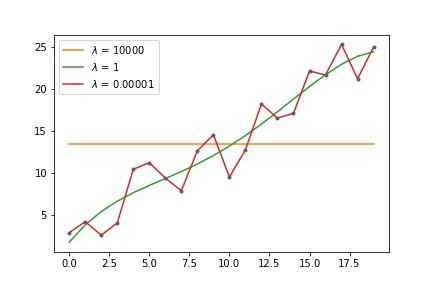
\includegraphics[width=0.5\paperwidth]{../LinearRegression/fig/diffregvalues_GEN.jpg}
    \caption{Effect of different regularization parameter values on final regression solution.}
    \label{fig:ridge-reg-diff-values}
\end{figure}

Notice how larger values of $\lambda$ produce less complex lines, which is the effect of applying more regularization. This is very nice for the problem we started with - which was wanting a way to choose which basis functions we wanted to use. With regularization, we can select many basis functions, and then allow regularization to `prune' the ones that aren't meaningful (by driving their weight parameters to 0). While this doesn't mean that we should use as many basis transformations as possible (there will be computational overhead for doing this), it does allow us to create a much more flexible linear regression model without creating a convoluted regression line.

\subsection{Bias-Variance Tradeoff and Decomposition}
Now that you know about regularization, you might have some intuition for why we need to find a balance between complex and simple regression solutions. A complex solution, while it might fit all of our training data, may not generalize well to future data points. On the other hand, a line that is too simple might not vary enough to provide good predictions at all. This phenomenon is not unique to linear regression- it's actually a very fundamental concept in machine learning that's known as the \textbf{bias-variance tradeoff}.

\begin{definition}{Bias-Variance Tradeoff}{bias-variance-tradeoff}
    When construction machine learning models, we have a choice somewhere on a spectrum between two extremes: fitting exactly to our training data or not varying in response to our training data at all. The first extreme, fitting all of our training data, is a situation of high \textit{variance}, because our output changes heavily in reponse to our input data (see the red line in Figure \ref{fig:ridge-reg-diff-values}). At the other extreme, a solution that doesn't change in response to our training data at all, is a situation of high \textit{bias}. This means that our target output doesn't fluctuate at all as a result of our training data.
\end{definition}

Obviously a good solution will fall somewhere in between these two extremes of total variance and total bias. Indeed, we have techniques like regularization that help us balance the two extremes, and we have additional techniques like \textit{cross-validation} that help us determine when we have found a good balance between the two.

\readernote{In case you are not familiar with the terms \textit{bias} and \textit{variance}, we provide their statistical definitions here:
\begin{align*}
    \text{bias($\theta$)} = \mathrm{E}[\theta] - \theta
\end{align*}
\begin{align*}
    \text{variance($\theta$)} = \mathrm{E}[(\theta - \mathrm{E}[\theta])^{2}]
\end{align*}
}

Before we discuss how to effectively balance these two outcomes, we will first show that the bias-variance tradeoff is not only conceptual but also has probabilistic underpinnings. Specifically, any loss that we can incur over our training set for a given model can be described in terms of bias and variance, as we will demonstrate now.

\begin{derivation}{Bias-Variance Decomposition}{bias-variance-decomp}
    Let's begin by asserting that we have a model $f(\cdot)$ that makes a prediction of our target $y$ given input data point $\textbf{x}$. We wish to break down the squared error of $f$ into terms involving bias and variance. \\

    Start with the expected squared error, where the expectation is taken with respect to both our data set $\textbf{D}$, which is composed of (\textbf{x}, $y$) pairs, and our conditional distribution of $y | \textbf{x}$:
    \begin{align*}
        \textit{MSE} = \mathrm{E}[(y - f(\textbf{x}))^{2}]
    \end{align*}
    For reasons that will become clear in a few steps, add and subtract our target mean, $\bar{y}$ inside of the squared term:
    \begin{align*}
        \textit{MSE} = \mathrm{E}[(y - \bar{y} + \bar{y} - f(\textbf{x}))^{2}]
    \end{align*}
    Group together the first two terms and the last two terms:
    \begin{align*}
        \textit{MSE} = \mathrm{E}[((y - \bar{y}) + (\bar{y} - f(\textbf{x})))^{2}]
    \end{align*}
    Expanding this expression and using linearity of expectation:
    \begin{equation} \label{bias-variance-intermediate-1}
        \textit{MSE} = \mathrm{E}[(y - \bar{y})^{2}] + \mathrm{E}[(\bar{y} - f(\textbf{x}))^{2}] + 2\mathrm{E}[(y - \bar{y})(\bar{y} - f(\textbf{x}))]
    \end{equation}
    Let's examine the last term, $2\mathrm{E}[(y - \bar{y})(\bar{y} - f(\textbf{x}))]$. Notice that $(\bar{y} - f(\textbf{x}))$ does not depend on the conditional distribution of $y|\textbf{x}$ at all. Thus, we are able to move one of those expecations in, which makes this term:
    \begin{align*}
        2\mathrm{E}[(y - \bar{y})(\bar{y} - f(\textbf{x}))] = 2\mathrm{E}_{D}[\mathrm{E}_{y|\textbf{x}}[(y - \bar{y})](\bar{y} - f(\textbf{x}))]
    \end{align*}
    And note that:
    \begin{align*}
        \mathrm{E}_{y|\textbf{x}}[(y - \bar{y})] = 0
    \end{align*}
    Which eliminates this last term entirely:
    \begin{align*}
        2\mathrm{E}[(y - \bar{y})(\bar{y} - f(\textbf{x}))] = 2\mathrm{E}_{D}[0 \cdot (\bar{y} - f(\textbf{x}))] = 0
    \end{align*}
    We can now write Equation \ref{bias-variance-intermediate-1} as:
    \begin{equation} \label{bias-variance-intermediate-2}
        \textit{MSE} = \mathrm{E}[(y - \bar{y})^{2}] + \mathrm{E}[(\bar{y} - f(\textbf{x}))^{2}]
    \end{equation}
    We now have two terms contributing to our squared error. We will ignore the first term $\mathrm{E}[(y - \bar{y})^{2}]$, as this is unidentifiable \textit{noise} in our data set. In other words, our data will randomly deviate from the mean in ways we cannot predict. On the other hand, we can work with the second term $\mathrm{E}[(\bar{y} - f(\textbf{x}))^{2}]$ as it involves our model function $f(\cdot)$ \\

    As before, for reasons of derivation that will become clear in a few steps, let's add and subtract the mean of our prediction, $\bar{f(\cdot)}$, inside this expression:
    \begin{align*}
        \mathrm{E}[(\bar{y} - f(\textbf{x}))^{2}] = \mathrm{E}[(\bar{y} - \bar{f}(\textbf{x}) + \bar{f}(\textbf{x}) - f(\textbf{x}))^{2}]
    \end{align*}
    Expanding this squared term, we have:
    \begin{align*}
        \mathrm{E}[(\bar{y} - f(\textbf{x}))^{2}] = (\bar{y} - \bar{f}(\textbf{x}))^{2} + \mathrm{E}[(\bar{f}(\textbf{x}) - f(\textbf{x}))^{2}] + 2\mathrm{E}[(\bar{y} - \bar{f}(\textbf{x}))(\bar{f}(\textbf{x}) - f(\textbf{x}))]
    \end{align*}
    As before, the third term here is 0:
    \begin{align*}
        2\mathrm{E}[(\bar{y} - \bar{f}(\textbf{x}))(\bar{f}(\textbf{x}) - f(\textbf{x}))] = 2(\bar{y} - \bar{f}(\textbf{x}))\mathrm{E}[(\bar{f}(\textbf{x}) - f(\textbf{x}))] = 2(\bar{y} - \bar{f}(\textbf{x}))(0) = 0
    \end{align*}
    Leaving us with these two terms:
    \begin{align*}
        \mathrm{E}[(\bar{y} - f(\textbf{x}))^{2}] = (\bar{y} - \bar{f}(\textbf{x}))^{2} + \mathrm{E}[(\bar{f}(\textbf{x}) - f(\textbf{x}))^{2}]
    \end{align*}
    Notice the form of these two terms. The first one, $(\bar{y} - \bar{f}(\textbf{x}))^{2}$, is the squared \textit{bias} of our model. The second one, $\mathrm{E}[(\bar{f}(\textbf{x}) - f(\textbf{x}))^{2}]$, is the \textit{variance} of our model:
    \begin{align*}
        \mathrm{E}[(y - f(\textbf{x}))^{2}] = \textit{bias}(f(\textbf{x}))^{2} + \textit{variance}(f(\textbf{x}))
    \end{align*}

    Thus, our total squared error, plugging in to Equation \ref{bias-variance-intermediate-2} can be written as:
    \begin{align*}
        \boxed{\textit{MSE} = \textit{noise}(\textbf{x}) + \textit{bias}(f(\textbf{x}))^{2} + \textit{variance}(f(\textbf{x}))}
    \end{align*}
\end{derivation}

The key takeaway of the bias-variance decomposition is that the controllable error in our model is given by the squared bias and variance. Holding our error constant, to decrease bias requires increasing the variance in our model, and vice-versa. In general, a graph of the source of error in our model might look something like this:

\begin{figure}
    \centering
    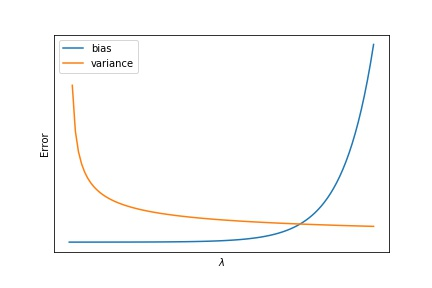
\includegraphics[width=0.5\paperwidth]{../LinearRegression/fig/biasvariance_GEN.jpg}
    \caption{Bias and variance both contribute to the overall error of our model.}
    \label{fig:bias-vs-variance}
\end{figure}

For a moment, consider what happens on the far left side of this graph. Our variance is very high, and our bias is very low. In effect, we're fitting perfectly to all of the data in our data set. This is exactly why we introduced the idea of regularization from before - we're fitting a very convoluted line that is able to pass through all of our data but which doesn't generalize well to new data points. There is a name for this phenomenon: \textbf{overfitting}.

\begin{definition}{Overfitting}{overfitting}
    A phenomenon where we construct a convoluted model that is able to predict every point in our data set perfectly but which doesn't generalize well to new data points.
\end{definition}

The opposite idea, \textbf{underfitting}, is what happens at the far right of the graph: we have high bias and aren't responding to the variation in our data set at all.

\begin{definition}{Underfitting}{underfitting}
    A phenomenon where we construct a model that doesn't respond to variation in our data at all.
\end{definition}

So you can hopefully now see that the bias-variance tradeoff is important to managing the problem of overfitting and underfitting. Too much variance in our model and we'll overfit to our data set. Too much bias and we won't account for the trends in our data set at all.

In general, we would like to find a sweet spot of moderate bias and variance that produces minimal error. In the next section, we will explore how we find this sweet spot.

\subsection{Cross-Validation}
We've seen that in choosing a model, we incur error that can be described in terms of bias and variance. We've also seen that we can regulate the source of error through regularization, where heavier regularization increases the bias of our model. A natural question then is how do we know how much regularization to apply to achieve a good balance of bias and variance?

Another way to look at this is that we've traded the question of finding the optimal number of basis functions for finding the optimal value of the regularization parameter $\lambda$, which can be seen as a slightly easier problem in most contexts.

One of the best solutions to finding the sweet spot for our regularization parameter, or any hyperparemter for that matter, is known as \textbf{cross-validation}.

\begin{definition}{Cross-Validation}{cross-validation}
    A subsampling procedure used over a data set to tune hyperparameters and avoid over-fitting. Some portion of a data set (10-20\% is common) is set aside, and training is performed on the remaining, larger portion of data. When training is complete, the smaller portion of data left out of training is used for testing. The larger portion of data is sometimes referred to as the \textit{training set}, and the smaller portion is sometimes referred to as the \textit{testing set}.
\end{definition}

Cross-validation is often performed more than once for a given setting of hyperparameters to avoid a skewed set of testing data occuring by change. In \textbf{K-Folds Cross-Validation}, you perform cross-validation \textbf{K} times, allocating $\frac{1}{\textbf{K}}$ of your data for the testing set at each iteration.

Let's tie this back into finding a good regularization parameter. For a given value of $\lambda$, we will incur a certain amount of error in our model. We can measure this error using cross-validation, where we train our model on the training set and compute the final error using the testing set. To find the optimal value for $\lambda$, we perform cross-validation using different values of $\lambda$, eventually settling on the value that produces the lowest final error. This will effectively trade off bias and variance, finding the value of $\lambda$ that minimizes the toal error.

You might wonder why we need to perform cross-validation at all - why can't we train on the entire data set and then compute the error over the entire data set as well?

The answer is \textit{overfitting}. If we train over the entire data set and then test our results on the exact same data set, we are likely to choose a regularization parameter that encourages our model to conform to the exact variation in our dataset instead of finding the generalizable trends. By training on one set of data, and then testing on a completely different set of data, we force our model to find good generalizations in our data set. This ultimately allows us to pick the regularization term $\lambda$ that finds the sweet spot between bias and variance, overfitting and underfitting.

\subsection{Bayesian Linear Regression}
We've thus far been discussing linear regression exclusively in terms of a loss function that helps us fit a set of weights to our data. In particular, we have been working with least squares, which has nice properties that make it a reasonable loss function.

In a very satisfying fashion, least squares also has a statistical foundation. In fact, you can recover the least squares loss function purely from a statistical derivation that we present here.

Consider our data set $\textbf{D} = \{(\textbf{x}_{i}, y_{i})\}_{i = 1}^{N}$, $\textbf{x}_{i} \in\mathbb{R}^m$, $y \in\mathbb{R}$. Let's imagine that our data was generated according to the following process:

\begin{align*}
    y_{i} \sim \mathcal{N}(\textbf{w}^{T}\phi(\textbf{x}_{i}), \beta^{-1})
\end{align*}

Which can be written equivalently as:

\begin{equation} \label{normal-over-w}
    p(y_{i} | \textbf{x}_{i}, \textbf{w}, \beta) = \mathcal{N}(\textbf{w}^{T}\phi(\textbf{x}_{i}), \beta^{-1})
\end{equation}

The interpretation of this is that our target value $y$ is generated according to some linear combination of our inputs \textbf{x}, but there is also some noise in the data generating process described by the variance parameter $\beta^{-1}$. This is exactly the same setup as before, except now we are acknowledging some noise in existing in our data.

\readernote{It's common to write variance as an inverse term, such as $\beta^{-1}$. The parameter $\beta$ is then known as the \textit{precision}, which is sometimes easier to work with than the variance.}

As before, we now ask the question: how do we solve for the optimal weights \textbf{w}? One approach we can take is to maximize the probability of observing our target data \textbf{Y}. This technique is known as \textit{maximum likelihood estimation}.

\begin{derivation}{Maximum Likelihood Estimation - Bayesian Linear Regression}{mle-bayesian}
    The likelihood of our data set is given by:

    \begin{align*}
        p(\textbf{Y} | \textbf{X}, \textbf{w}, \beta) = \prod_{i=1}^{N} \mathcal{N}(\textbf{w}^{T}\phi(\textbf{x}_{i}), \beta^{-1})
    \end{align*}
    We then take the logarithm of the likelihood, and since the logarithm is a strictly increasing, continuous function, this will not change our optimal weights \textbf{w}:
    \begin{align*}
        \ln{p(\textbf{Y} | \textbf{X}, \textbf{w}, \beta)} = \sum_{i=1}^{N} \ln{\mathcal{N}(\textbf{w}^{T}\phi(\textbf{x}_{i}), \beta^{-1})}
    \end{align*}
    Using the density function of a univariate Gaussian:
    \begin{align*}
        \ln{p(\textbf{Y} | \textbf{X}, \textbf{w}, \beta)} = \sum_{i=1}^{N} \ln{\frac{1}{\sqrt{2\pi\beta^{-1}}} e^{-(y_{i} - \textbf{w}^{T}\phi(\textbf{x}_{i}))^2 / 2\beta^{-1}}}
    \end{align*}
    \begin{align*}
        \ln{p(\textbf{Y} | \textbf{X}, \textbf{w}, \beta)} = \frac{N}{2}\ln{\beta} - \frac{N}{2}\ln{(2\pi)} - \frac{\beta}{2} \sum_{i=1}^{N} (y_{i} - \textbf{w}^{T}\phi(\textbf{x}_{i}))^2
    \end{align*}
    Notice that this is a quadratic function in \textbf{w}, which means that we can solve for it by taking the derivative with respect to \textbf{w}, setting that expression to 0, and solving for \textbf{w}:
    \begin{align*}
        \frac{\partial \ln{p(\textbf{Y} | \textbf{X}, \textbf{w}, \beta)}}{\partial \textbf{w}} = \beta \sum_{i=1}^{N} (y_{i} - \textbf{w}^{T}\phi(\textbf{x}_{i}))\phi(\textbf{x}_{i})^{T}
    \end{align*}
    \begin{align*}
        0 = \beta \sum_{i=1}^{N} (y_{i} - \textbf{w}^{T}\phi(\textbf{x}_{i}))\phi(\textbf{x}_{i})^{T}
    \end{align*}
    \begin{align*}
        0 = \sum_{i=1}^{N} y_{i}\phi(\textbf{x}_{i})^{T} - \textbf{w}^{T} \sum_{i=1}^{N} \phi(\textbf{x}_{i})\phi(\textbf{x}_{i})^{T}
    \end{align*}
    Notice that this is exactly the same form as Equation \ref{least-squares-solving-for-w}. Solving for \textbf{w} as before:
    \begin{align*}
        \textbf{w}^{*} = (\phi(\textbf{X})^{T}\phi(\textbf{X}))^{-1}\phi(\textbf{X})^{T}\textbf{Y}
    \end{align*}
    Note that you'll often see $\textbf{X} = \boldsymbol{\Phi}$, which is known as the design matrix, giving us:
    \begin{equation} \label{bayesian-solved-for-w}
        \textbf{w}^{*} = (\boldsymbol{\Phi}^{T}\boldsymbol{\Phi})^{-1}\boldsymbol{\Phi}^{T}\textbf{Y}
    \end{equation}
\end{derivation}

Notice that our final solution is exactly the same form as the solution in Equation \ref{least-squares-solved-for-w}, which we solved for by minimizing the least squares loss! \textbf{The takeaway here is that minimizing a least squares loss function is equivalent to maximizing the probability under the assumption of a linear model with Gaussian noise}.

\subsection{Regularization Interpretation}
We've thus far only discussed one form of regularization: ridge regression. Remember that under ridge regression, the loss function takes the form:

\begin{align*}
    \mathcal{L}(\textbf{w}) = \frac{1}{2} \sum_{i=1}^{n} (t - \textbf{w}^{T}\boldsymbol{\phi})^2 + \frac{\lambda}{2}\textbf{w}^{2}
\end{align*}

Where the $\frac{\lambda}{2}\textbf{w}^{2}$ term is for the regularization. We can generalize our type of regularization by writing it as:

\begin{align*}
    \mathcal{L}(\textbf{w}) = \frac{1}{2} \sum_{i=1}^{n} (t - \textbf{w}^{T}\boldsymbol{\phi})^2 + \frac{\lambda}{2}\big|\textbf{w}\big|^{h}
\end{align*}

where $h$ determines the type of regularization we are using and thus the form of the optimal solution that we recover.

The three most commonly used forms of regression are Lasso regression, ridge regression, and Elastic Net.

\subsubsection{Ridge Regression}
This is the case of $h = 2$, which we've already discussed, but what type of solutions does it tend to uncover? Ridge regression prevents any individual weight from growing too large, providing us with solutions that are generally moderate.

\subsubsection{Lasso Regression}
Lasso regression is the case of $h = 1$. Unlike ridge regression, Lasso regression will drive some parameters $\textbf{w}_{i}$ to zero if they aren't informative for our final solution. Thus, Lasso regression is good if you wish to recover a sparse solution that will allow you to throw out some of your basis functions.

You can see the forms of ridge and lasso regression in Figure \ref{fig:ridge-and-lasso-reg-fn-form}.

\begin{figure}
    \centering
    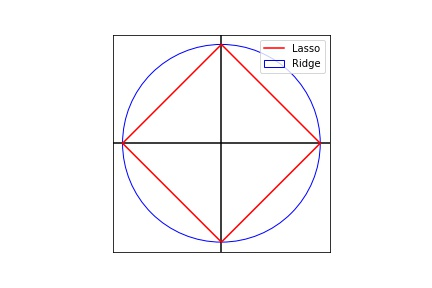
\includegraphics[width=0.5\paperwidth]{../LinearRegression/fig/ridgeandlassoreg_GEN.jpg}
    \caption{Form of the ridge (blue) and lasso (red) regression functions.}
    \label{fig:ridge-and-lasso-reg-fn-form}
\end{figure}

\subsubsection{Elastic Net}
Elastic Net is a middle ground between ridge and Lasso regression, which it achieves by using a linear combination of the respective regularization terms. Depending on how heavily each regularization term is weighted, this can produce results on a spectrum between Lasso and ridge regression. \\

\subsection{Bayesian Regularization} \label{bayesian-regularization-section}
We've seen regularization in the context of loss functions, where the goal is to penalize large weight values. How does the concept of regularization apply to Bayesian linear regression?

The answer is that we can interpret regularizing out weight parameters as adding a prior distribution over \textbf{w}.

\begin{derivation}{Bayesian Regularization Derivation}{bayesian-regularization-derivation}
    Because we wish to shrink our weight values toward 0, we will select a Normal prior with mean 0 and variance $\boldsymbol{S}_{0}^{-1}$:
    \begin{align*}
        \textbf{w} \sim \mathcal{N}(0, \boldsymbol{S}_{0}^{-1}\textbf{I})
    \end{align*}
    Remember that the distribution over our observed data is Normal as well from Equation \ref{normal-over-w}, written here in terms of our entire data set:
    \begin{align*}
        p(\textbf{Y} | \textbf{X}, \textbf{w}, \beta) = \mathcal{N}(\textbf{X}\textbf{w}, \beta^{-1}\textbf{I})
    \end{align*}
    We want to combine the likelihood and the prior to recover the posterior distribution of $\textbf{w}$, which follows directly from Bayes' Theorem:
    \begin{align*}
        p(\textbf{w}|\textbf{X},\textbf{Y}, \beta) \propto p(\textbf{Y}| \textbf{X}, \textbf{w}, \beta)p(\textbf{w})
    \end{align*}
    We now wish to find the value of \textbf{w} that maximizes the posterior distribution. We can maximize the log of the posterior with respect to \textbf{w}, which simplifies the problem slightly:
    \begin{align*}
        \ln{p(\textbf{w}|\textbf{X},\textbf{Y}, \beta)} \propto \ln{p(\textbf{Y}| \textbf{X}, \textbf{w}, \beta)} + \ln{p(\textbf{w})}
    \end{align*}
    Let's handle $\ln{p(\textbf{Y}| \textbf{X}, \textbf{w}, \beta)}$ first:
    \begin{align*}
        \ln{p(\textbf{Y}| \textbf{X}, \textbf{w}, \beta)} &= \ln{\prod_{i=1}^{N} \mcN(y_{i} | \textbf{w}^{T} \textbf{x}_{i}, \beta^{-1})} \\
        &= \ln{\prod_{i=1}^{N} \frac{1}{\sqrt{2\pi\beta^{-1}}} \exp{\bigg\{-\frac{\beta}{2}(y_{i} - \textbf{w}^{T} \textbf{x}_{i})^2\bigg\}}} \\
        &= \textbf{C} -\frac{\beta}{2}\sum_{i=1}^{N} (y_{i} - \textbf{w}^{T} \textbf{x}_{i})^2 + \frac{1}{\sqrt{2\pi\beta^{-1}}}
    \end{align*}
    where \textbf{C} collects the constant terms that don't depend on \textbf{w}. Let's now handle $\ln{p(\textbf{w})}$:
    \begin{align*}
        \ln{p(\textbf{w})} &= \ln{\mathcal{N}(0, \boldsymbol{S}_{0}^{-1}\textbf{I})} \\
        &= \ln{\frac{1}{(|2\pi\boldsymbol{S}_{0}^{-1}\textbf{I}|)^{\frac{1}{2}}} \exp{\bigg\{-\frac{\boldsymbol{S}_{0}}{2} \textbf{w}^{T}\textbf{w}\bigg\}}} \\
        &= \textbf{C} -\frac{\boldsymbol{S}_{0}}{2} \textbf{w}^{T}\textbf{w}
    \end{align*}
    combining the terms for $\ln{p(\textbf{Y}| \textbf{X}, \textbf{w}, \beta)}$ and $\ln{p(\textbf{w})}$:
    \begin{align*}
        \ln{p(\textbf{w}|\textbf{X},\textbf{Y}, \beta)} = -\frac{\beta}{2}\sum_{i=1}^{N} (y_{i} - \textbf{w}^{T} \textbf{x}_{i})^2 - \frac{\boldsymbol{S}_{0}}{2} \textbf{w}^{T}\textbf{w}
    \end{align*}
    dividing by a positive constant $\beta$:
    \begin{align*}
        \ln{p(\textbf{w}|\textbf{X},\textbf{Y}, \beta)} = -\frac{1}{2}\sum_{i=1}^{N} (y_{i} - \textbf{w}^{T} \textbf{x}_{i})^2 - \frac{\boldsymbol{S}_{0}}{\beta}\frac{1}{2} \textbf{w}^{T}\textbf{w}
    \end{align*}
    Notice at this point that maximizing the posterior probability is equivalent to minimizing the sum of squared errors $(y_{i} - \textbf{w}^{T} \textbf{x}_{i})^2$ and the regularization term $\textbf{w}^{T}\textbf{w}$.
\end{derivation}

\textbf{The interpretation of this is that adding a prior over the distribution of our weight parameters \textbf{w} is equivalent to adding a regularization term where $\lambda = \frac{\boldsymbol{S}_{0}}{\beta}$}

\subsection{Predictive Distribution}
Remaining in the setting of Bayesian Linear Regression, we may wish to get a distribution over our weights $\textbf{w}$ instead of a point estimator for it using maximum likelihood. As we saw in Section \ref{bayesian-regularization-section}, we can introduce a prior distribution over $\textbf{w}$, then together with our observed data, we can produce a posterior distribution over $\textbf{w}$ as desired.

\begin{derivation}{Posterior Predictive Derivation}{posterior-predictive-derivation}
    For the sake of simplicity and ease of use, let's make our prior over $\textbf{w}$ a Normal distribution with mean $\boldsymbol{\mu}_{0}$ and variance $\boldsymbol{S}_{0}^{-1}$:
    \begin{align*}
        p(\textbf{w}) = \mathcal{N}(\boldsymbol{\mu}_{0}, \boldsymbol{S}_{0}^{-1})
    \end{align*}
    Remembering that the observed data is normally distributed, and accounting for Normal-Normal conjugacy, our posterior distribution will be a Normal as well:
    \begin{align*}
        p(\textbf{w}|\textbf{X},\textbf{Y}, \beta) = \mathcal{N}(\boldsymbol{\mu}_{N}, \boldsymbol{S}_{N}^{-1})
    \end{align*}
    where
    \begin{align*}
        \boldsymbol{S}_{N} = (\boldsymbol{S}_{0}^{-1} + \beta\textbf{X}^{T}\textbf{X})^{-1} \\
        \boldsymbol{\mu}_{N} = \boldsymbol{S}_{N}(\boldsymbol{S}_{0}^{-1}\boldsymbol{\mu}_{0} + \beta\textbf{X}\textbf{Y})
    \end{align*}

    We now have a posterior distribution over \textbf{w}. However, usually this distribution is not what we care about. We're actually interested in making a point prediction for the target $y^{*}$ given a new input $\textbf{x}^{*}$. How do we go from a posterior distribution over \textbf{w} to this prediction? \\

    The answer is using what's known as the posterior predictive over $y^{*}$ given by:
    \begin{equation}
    \begin{split}
        p(y^{*} | \textbf{x}^{*}, \textbf{X}, \textbf{Y}) = \int_{\textbf{w}} p(y^{*} | \textbf{x}^{*}, \textbf{w})p(\textbf{w} | \textbf{X}, \textbf{Y})d\textbf{w} \\
        = \mathcal{N}(y^{*} | \textbf{w}^{T}\textbf{x}^{*}, \beta^{-1})\mathcal{N}(\textbf{w} | \boldsymbol{\mu}_{N}, \boldsymbol{S}_{N}^{-1})d\textbf{w}
    \end{split}
    \end{equation}
\end{derivation}

\textbf{The idea here is to average the probability of $y^{*}$ over all the possible setting of \textbf{w}, weighting the probabilities by how likely each setting of \textbf{w} is according to its posterior distribution.}

\section{Practice Problems}